\documentclass[10pt,xcolor=svgnames]{beamer} %Beamer
\usepackage{palatino} %font type
\usepackage{xcolor}
\usepackage[font={tiny}]{caption}
\usefonttheme{metropolis} %Type of slides
\usefonttheme[onlymath]{serif} %font type Mathematical expressions
\usetheme[progressbar=frametitle,titleformat frame=smallcaps,numbering=counter]{metropolis} %This adds a bar at the beginning of each section.
\useoutertheme[subsection=false]{miniframes} %Circles in the top of each frame, showing the slide of each section you are at

\usepackage{appendixnumberbeamer} %enumerate each slide without counting the appendix

\definecolor{SysBlue}{RGB}{12,120,183}
\definecolor{Progress}{RGB}{56,60,92}
\definecolor{Header}{RGB}{12,120,183}
\definecolor{SlideTitle}{RGB}{0,137,208}
\definecolor{ToC}{RGB}{51,58,66}

\setbeamercolor{progress bar}{fg=Progress} %These are the colours of the progress bar. Notice that the names used are the svgnames
\setbeamercolor{title separator}{fg=SysBlue} %This is the line colour in the title slide
\setbeamercolor{structure}{fg=black} %Colour of the text of structure, numbers, items, blah. Not the big text.
\setbeamercolor{normal text}{fg=black!87} %Colour of normal text
\setbeamercolor{alerted text}{fg=DarkRed!60!Gainsboro} %Color of the alert box
\setbeamercolor{example text}{fg=ToC} %Colour of the Example block text
\setbeamercolor{background canvas}{bg=white}


\setbeamercolor{palette primary}{bg=SlideTitle, fg=white} %These are the colours of the background. Being this the main combination and so one. 
\setbeamercolor{palette secondary}{bg=Header, fg=white}
\setbeamercolor{palette tertiary}{bg=Header, fg=white}
\setbeamercolor{section in toc}{fg=ToC} %Color of the text in the table of contents (toc)

%These next packages are the useful for Physics in general, you can add the extras here. 
\usepackage{amsmath,amssymb}
\usepackage{slashed}
\usepackage{cite}
\usepackage{relsize}
\usepackage{caption}
\usepackage{subcaption}
\usepackage{multicol}
\usepackage{booktabs}
\usepackage[scale=2]{ccicons}
\usepackage{pgfplots}
\usepgfplotslibrary{dateplot}
\usepackage{geometry}
\usepackage{xspace}
\usepackage{enumitem}
\newcommand{\themename}{\textbf{\textsc{bluetemp}\xspace}}%metropolis}}\xspace}

\title{DAOSYS}
\author[Name]{Ian Moore, PhD \inst{$\dagger$} and Cyotee Doge \inst{$\dagger\dagger$}}%With inst, you can change the institution they belong
\subtitle{Smart DAO Protocol for Decentralized Finance}

\institute[shortinst]{\inst{$\dagger$} Syscoin Researcher, Syscoin Platform (email: imoore@syscoin.org) \and %
                      \inst{$\dagger\dagger$} DAO Advisor, Syscoin Platform (email: cyotee@syscoin.org)}

\date{October 27, 2022} %Here you can change the date
\titlegraphic{\vspace{-0.5cm}\hfill
\includegraphics[scale=0.23]{logo.png}} %You can modify the location of the logo by changing the command \vspace{}. 

\begin{document}
{
\setbeamercolor{background canvas}{bg=white, fg=black}
\setbeamercolor{normal text}{fg=black}
\maketitle
}%This is the colour of the first slide. bg= background and fg=foreground

\metroset{titleformat frame=smallcaps} %This changes the titles for small caps

\begin{frame}{Outline}
  \setbeamertemplate{section in toc}[sections numbered] %This is numbering the sections
  \tableofcontents[hideallsubsections] %You can comment this line if you want to show the subsections in the table of contents
\end{frame}

\begin{frame}{Objectives}

\metroset{block=fill}
\begin{exampleblock}{\textsc{First ever smart DAO protocol}}
\begin{itemize}
  \item Similar to Ethereum in the sense that both protocols work with decentralized immutable storage
  \item Instead launching contracts from chains, we work with Diamonds
\end{itemize}  
\end{exampleblock}

\begin{exampleblock}{\textsc{Self-sovereign capital coordination}}
\begin{itemize}
  \item Does this via its new Autonomous Service Engine technology
  \item Made possible through an extension of the multi-facet proxy called Diamonds outlined in EIP-2535
\end{itemize}
\end{exampleblock}

\begin{exampleblock}{\textsc{Masternode Yield Farming}}
\begin{itemize}
  \item First of a new class of DAOs
  \item System of trustlessly investing Masternode yields into a DeFi liquidity provider
\end{itemize}
\end{exampleblock}

\end{frame}


\section{Introduction}

\begin{frame}{Introduction: Overview} %You can change fragile by standout


The features that DAOSYS will have are as follows:

\begin{itemize}
  \item[$\diamond$] Smart DAO protocol via hyper-diamond proxy
  \item[$\diamond$] Self-sovereign via trustless automatic integration
  \item[$\diamond$] Seamless fast deployment using secure templates
  \item[$\diamond$] Hyper-diamond standard
  \item[$\diamond$] Collateralized VE (vesting) indexing token
  \item[$\diamond$] Automated audits of child DAOs
  \item[$\diamond$] Fully backed (eg, DAI, SYS)
  \item[$\diamond$] Non-speculative asset
  \item[$\diamond$] No code or low code deployments via user interface
  \item[$\diamond$] New emergent behavior and innovation for DeFi
\end{itemize}  

\end{frame}


\begin{frame}{Introduction: Smart DAO protocol} %You can change fragile by standout

\begin{figure}[h!]
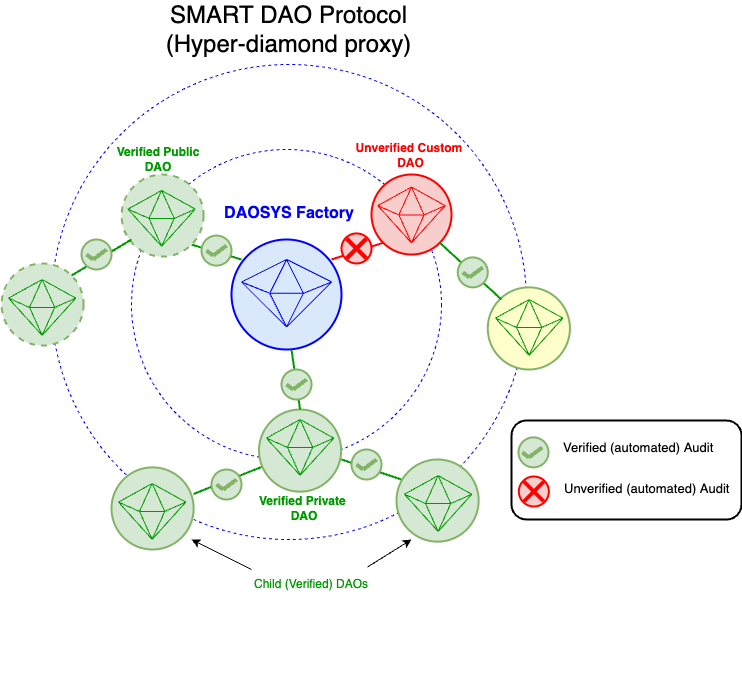
\includegraphics[width=3in]{img/smart_dao.png}
\caption{DAOSYS as the smart DAO protocol, utilizing the hyper-diamond proxy; see EIP-2535} 
\label{fig:daosys_protocol}
\end{figure}

\end{frame}

\begin{frame}{Introduction: Security}

When a DAO joins the DAOSYS ecosystem it will be either verified or unverified, which is a security attribute that will dictate the way it conducts itself on the network

\begin{itemize}
  \item[$\diamond$] \textbf{Public-verified}: most common type of DAO on the network and are essentially clones of DAOSYS
  \item[$\diamond$] \textbf{Public-unverified}: second most adopted usecase on the network having freedoms akin to a Redhat or AWS EC2 licence agreement
  \item[$\diamond$] \textbf{Private-verified}: may be used as a public testnet to vet new ideas that are uncommon to the network
  \item[$\diamond$] \textbf{Private-unverified}: may be useful to those looking setup smart wallets with modules consisting of a host of sophisticated asset managing DeFi strategies
\end{itemize} 
\end{frame}

\section{Governance}


\begin{frame}{Governance} 

A user creates a DAO by selecting which vaults and bond markets they would like to include. These vaults may come from one of four sources:

\begin{itemize}
  \item[$\diamond$] Reuse an existing vault
  \item[$\diamond$] Recreate an existing vault
  \item[$\diamond$] New pool with new investment strategy
  \item[$\diamond$] New pool with custom code
\end{itemize} 

\end{frame}

\begin{frame}{Governance:  New pool with custom code} 

\begin{figure}[h!]
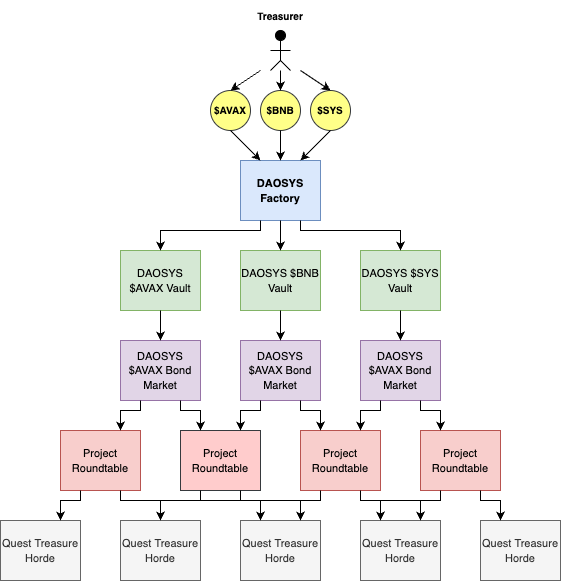
\includegraphics[width=2.3in]{img/governance.png}
\caption{DAOSYS Governance Structure: new pool with custom code (ie, Quests)} 
\label{fig:daosys_governance}
\end{figure}

\end{frame}

\section{Architecture}

\begin{frame}{Architecture: Structure of the Hyper-diamond standard}

Three-tier architecture is a well-established software architecture that organizes backend applications into three logical computing tiers, which include:

\begin{itemize}
  \item[$\diamond$] Presentation tier: controller classes
  \item[$\diamond$] Application tier: services classes
  \item[$\diamond$] Data tier: repository classes
\end{itemize} 

The utility of this is to manage properly structured code to make it easier for other developers to work with. Thus, no matter what the application (eg, API, CLI, etc.), it is important to approach software design in this way, which is what we are introducing into our DAOSYS smart contract implementations, namely the Hyper Diamond Standard.

\end{frame}


\begin{frame}{Architecture: DAOSYS package}

\begin{figure}[h!]
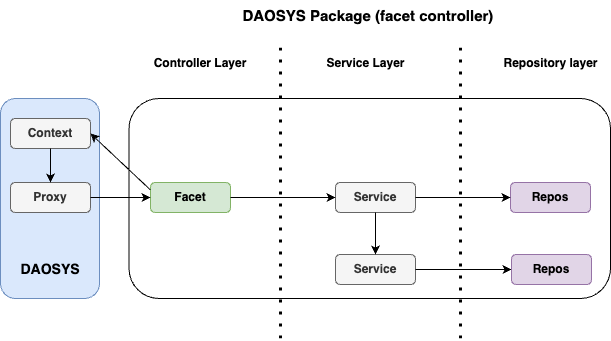
\includegraphics[width=3in]{img/three_tier_package.png}
\caption{Three-tier structure of the DAOSYS package} 
\label{fig:daosys_governance}
\end{figure}

\end{frame}




\section{Tokenomics}

\begin{frame}{Tokenomics: General Model}

\begin{figure}[h!]
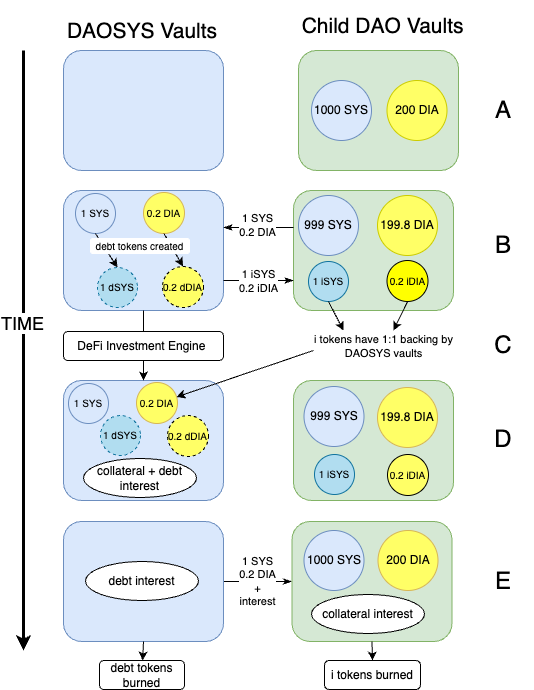
\includegraphics[width=2in]{img/tokenomics_model.png}
\caption{Tokenomics model representing minimum commitment of publicly and privately verified child DAOs} 
\label{fig:tokenomics_model}
\end{figure}

\end{frame}

\begin{frame}{Tokenomics: Basic Steps}

The five steps of the tokenomics model described in Fig. \ref{fig:tokenomics_model} are as follows:

\begin{enumerate}[label=\Alph*]
  \item Initially assume DAOSYS vaults contains no assets
  \item Triggering event stimulates a small deposit from the Child DAO vaults into the DAOSYS vaults
  \item DAOSYS will send both these debt and collateral tokens through a DeFi investment engine
  \item DAOSYS vault will collect interest from these newly acquired collateral and debt assets
  \item Child DAO recalls the original collateral and all its earned interest, while DAOSYS keeps the debt interest
\end{enumerate} 

\end{frame}


\begin{frame}{Tokenomics: Simulator}

\begin{figure}[h!]
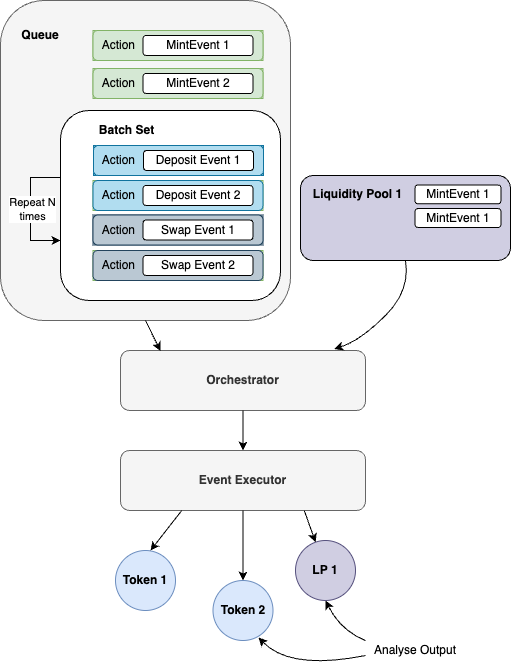
\includegraphics[width=2in]{img/simulator.png}
\caption{System components to DeFi Python simulator for DAOSYS} 
\label{fig:daosys_simulator}
\end{figure}

\end{frame}


\begin{frame}{Tokenomics: Simulator (2)}

\begin{table}[h]
\tiny
\centering
\begin{tabular}{ |l|l| } 
\hline
 \textbf{Simulator Component} & \textbf{Description} \\
\hline
Agents          & Entities that engage with the system, and are  \\
                & subcategorized into tokens and users \\
Events          & Agnostic events that take place within the \\ 
				& system (eg, mint, deposit, withdraw, swap, \\
				& and rebase) \\
ModelQueue      & Queue of univariate events that are modelled \\
				& aprior that can be fed into the system as \\
				& events\\
Actions         & Event actions that are fed into the system \\
				& performed by agents; they can either be single \\
				& stand-alone independent event actions or \\
				& chained together with dependency \\
ActionChains    & Actions that have dependencies on other \\
				& actions as inputs \\				
ActionBatch     & Batches of actions placed together into a \\
				& repeatable sequence; there is only one \\
				& assigned time delta per the pass of each batch, \\
				& and there is no limit as to the number of \\
				& batches that can be created \\
Liquidity Pools & Pool of two token agents managed by constant \\ 
				& product trading \\
Orchestrator    & Manages agents and actions working within the \\ 
				& system \\
Event Queue     & Queue of storable actions \\
Event Executor  & Final step which executes queue of action \\
				& events \\
\hline
\end{tabular}
\caption{Descriptions of DeFi python simulator components; refer to Fig. \ref{fig:daosys_simulator} to see how components interact with one another.}
\label{table:simulator_components}
\end{table}

\end{frame}

\section{Roadmap}

\begin{frame}{Roadmap: Expectations}

Prior to mainnnet release:

\begin{itemize}
  \item[$\diamond$] Syscoin's L2 (ie, Rollux) must launch first along with Syscoin's Proof-of-Data Availability (PoDA)
  \item[$\diamond$] It is our intention that DAOSYS be launched when Rollux goes live
  \item[$\diamond$] We are expecting to launch DAOSYS in the early part of 2023 with crypto's first Masternode Yield Farm as its first functioning child DAO
\end{itemize} 

\end{frame}


\begin{frame}{Roadmap: Usecases}

Explored usecases:

\begin{itemize}
  \item[$\diamond$] \textbf{Masternode Yield Farming}: Syscoin plans to incentivize Masternode operators where they can put yields to work by investing them into a DeFi liquidity provider which will be automated in a trustless manner through DAOSYS
  \item[$\diamond$] \textbf{Index Tokens (Crypto ETFs)}: since DAOSYS itself is a non-speculated asset backed index of cryptos, for the first time we introduce a new class of cryptos called index tokens or crypto ETFs. The intelligence of the DAOSYS protocol will allow for the seamless, secure deployment of these index tokens using one of its readily available templates addressing this important usecase.
\end{itemize} 

\end{frame}



\begin{frame}[standout]
  Thank you! 
\end{frame}



\end{document}